\section{Preliminary Work}
\label{sec:preliminary}
%\emph{\color{red}Preliminary work section that describes the system you have built so far and/or preliminary results you have collected. Describe the strengths and weaknesses of your approach to date, including what it can and cannot do (or in the case of results, what those results show and what are the limitations of your results).}

In this section, we describe our preliminary work building an experimental 802.11n platform, in particular a tool that uses commodity Intel Wi-FI NICs to measure the 802.11n Channel State Information. Next, we use measurements of packet delivery vs RSSI and CSI to show explain why RSSI fails to predict packet delivery in real wireless channels. When then use CSI in conjunction with the concept of an Effective SNR for wireless links to explain the performance of links that experience frequency-selective fading. We demonstrate experimentally that CSI and Effective SNR can predict the performance of wireless links across a wide range of configurations, such as rate selection and transmit power control. Finally, we present trace-driven simulation results that show that a simple Effective SNR-based rate \emph{selection} (not \emph{adaptation}) can be used to achieve good performance in varying channels.

\subsection{802.11n CSI Tool and Experimental Platform}
\label{sec:platform}
In conjunction with Intel Labs Seattle, we have built an experimental 802.11n platform that uses the Intel Wi-Fi Wireless Link 5300 (\term{iwl5300}) 802.11a/b/g/n network cards. We modified the closed-source firmware and open-source Linux driver to add a number of experimental features importantly to measure the 802.11n CSI. Here, we summarize these features.

\heading{802.11n CSI Measurement.} The channel sounding mechanism added in 802.11n defines a management frame used to report the CSI from the receiver of a frame back to the transmitter. This mechanism is intended for calibration or to inform transmit beamforming, and we co-opt it for our experiments. We configure the NIC with a debug mode to compute this feedback packet for every received frame,\footnote{CSI is reported for correctly received frames destined for the measurement node or sent to a special hard-coded broadcast address.} rather than just during sounding, and send it up to the driver instead of back to the transmitter. The \term{iwl5300} provides CSI in a format that reports the channel matrices for 30 subcarrier groups, which is about one group for every 2 subcarriers at 20\MHz or every 4 subcarriers at 40\MHz. Each channel matrix entry is a complex number, with signed 8-bit resolution each for the real and imaginary parts. It specifies the gain and phase of the spatial path between a single transmit-receive antenna pair. Intel's implementation of the 802.11n CSI does not include per-subcarrier noise measurements, so we assume the noise floor is uniform across all subcarriers to compute SNRs. This is consistent with white noise observed on other OFDM platforms~\cite{Rahul_FARA}.

\heading{RSSI Measurement.} 
For each received packet the NIC reports the traditional metrics of RSSI per receive antenna, noise floor and the setting on the automatic gain controlled (AGC) amplifier. These combine to define the per-receive-chain packet SNR ($\rho_{\text{packet}}$):
\begin{equation}
\label{eq:per_chain_snr}
	\rho_{\text{packet}} = \text{RSSI (dBm)} - \text{Noise (dBm)} - \text{AGC (dB)}
\end{equation}
The \term{iwl5300} calculates the quantities RSSI and Noise as the respective sums of average signal strength and average error vector magnitude in each OFDM subcarrier~\cite{iwlwifi}. This is exactly the traditional definition of SNR applied to OFDM\@.

\heading{Transmit Power Control.} Our hardware enables us to vary the transmit power level from $-$10\dBm~(100\uW) to $+$16\dBm~(40\mW) in steps of 0.5\dB, and divides power equally across streams. Additionally, the \term{iwl5300} reduces the transmit power slightly when using the highest single-stream rates to avoid distortions caused by passing QAM-64 symbols with high peak-to-average power ratio through the transmit amplifier.

\heading{Rapid Rate Variation.} In normal operation, the \term{iwl5300} decouples queuing packets for transmission from selecting rates for these packets, since queues must be kept large to take advantage of 802.11n block transmissions. This makes it difficult to control the rate at which individual packets are transmitted. We modified the firmware and driver to support the transmission of individual packets at predetermined rates, and added driver-level code to rapidly iterate through a user-configurable set of available rates.

\heading{Userspace Connector.} We used the Linux kernel \term{connector} framework to implement a low-latency socket-based communication channel between the kernel driver and userspace utilities. This enables userspace utilities to logging of CSI and other output from the driver, and send messages that, e.g., change the currently selected rate or antennas or change the transmit power level.

\heading{Publicly Released Tool.} We have publicly released our experimental platform and CSI collection tool in the form of open source drivers, userspace utilities, MATLAB code, and binary firmware image~\cite{halperin_csitool}. At the time of writing, we are aware of several users, including multiple research and product groups within Intel, industrial researchers at HP Labs, and academic researchers at UT Austin, CMU, UCL, and the Hong Kong University of Science and Technology.

%The mechanisms we intend to use to for improving performance, flexibility, and reliability in wireless systems rely on finding good operating points in a large search space. For instance, as a device moves through the home, it might concurrently choose between different link rates, different numbers of spatial streams, multiple transmit or receive antennas, and possible intermediaries. It is important to converge to a solution quickly or the network will be unreliable and have low performance. As we will show, accurate physical layer measurements can help guide this search. We first describe the poor state of RF measurements in Wi-Fi today, and then describe our recent work to build a prototype that measures 802.11n CSI.

\subsection{Motivation: Inadequacy of RSSI}
\begin{figure}[t!]
	\centering
		\subfigure[A wired 802.11n link with variable attenuation has a predictable relationship between SNR and packet reception rate (PRR) and clear separation between rates.\vspace{-3pt}]{
			\label{fig:snr_prr_attenuator}
			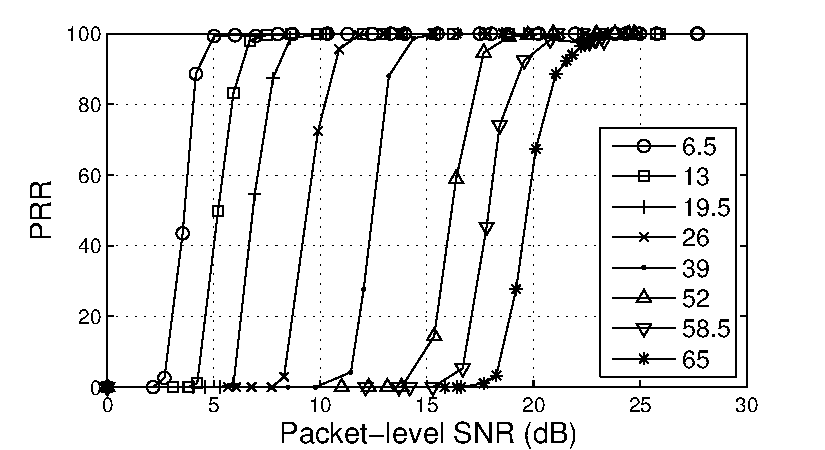
\includegraphics[width=2.7in,viewport=13 0 364 204,clip]{figures/embed_attenuator_snr_prr.pdf}
		}
%
      	\subfigure[Over real wireless channels in our testbeds, the transition region varies up to 10\dB. This loses the clear separation between rates (and so only three rates are shown for legibility).\vspace{-3pt}]{
			\label{fig:snr_prr_26_65}
			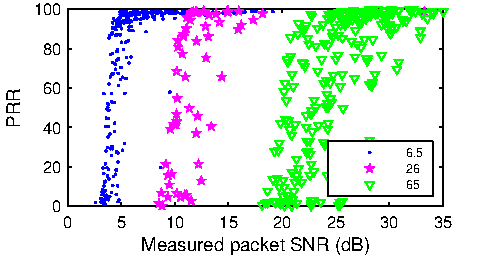
\includegraphics[width=2.8in,viewport=2 0 217 124,clip]{figures/embed_scatterplot_meas_snr_small.pdf}
		}
%
	\caption{\label{fig:rssi_predictions}Measured (single antenna) 802.11n packet delivery over wired and real channels.}%
\end{figure}
\topheading{Packet Delivery versus RSSI/SNR\@.}
Textbook analyses of modulation schemes give delivery probability for a single signal in terms of the signal-to-noise (SNR) ratio~\cite{Goldsmith}, %The SNR is defined as the ratio of the signal power to the thermal noise power, typically expressed on a logarithmic scale in decibels, i.e., SNR = $10\log_{10}(S/N)$. 
typically expressed on a log scale in decibels.
This model holds for narrowband channels with additive white Gaussian noise. It predicts a sharp transition region of 1--2\dB over which a link changes from extremely lossy to highly reliable. This makes the SNR a valuable indicator of performance.

We generated performance curves using SNR for the \term{iwl5300} over a simple wired link with a variable attenuator and for a single transmit and receive antenna. The result is shown for all single antenna 802.11n rates in \figref{fig:snr_prr_attenuator}. 
We observe a characteristic sharp transition region for packet reception rate (PRR) versus SNR\@. This is despite the relatively wide 20\MHz channel, 56 OFDM subcarriers, coding and other bit-level operations. This is the behavior we want from a link metric in order to predict packet delivery.

In contrast, packet delivery over real wireless channels does not exhibit the same picture. \figref{fig:snr_prr_26_65} shows the measured PRR versus SNR for three sample rates (6.5, 26, and 65\Mbps) over all wireless links in our testbeds, using the same 802.11n NICs. The SNR of the transition regions can exceed 10\dB, so that some links easily work for a given SNR and others do not. There is no longer clear separation between rates. This is consistent with other reported measurements that show RSSI does not predict packet delivery for real links~\cite{aguayo_roofnet, reis_sigcomm06, snr_infocom08, zhao_sensys03}.

\begin{figure}[t]
  \centering
  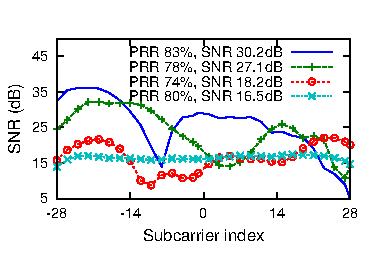
\includegraphics[width=\columnwidth,viewport=2 9 185 108,clip]{figures/embed_fsf-shape-two-links.pdf}
% viewport=2 10 170 108
  \caption{Channel gains on four links that perform about equally well at 52\Mbps. The more faded links require larger RSSIs (i.e., more transmit power) to achieve similar PRRs.}
  \label{fig:example_fsf_shape}
  % information for the links used to make above plot: 
  %srcs = [1 10 3 3];
  %dests = [9 11 2 5];
  %txpowers = [-4 20 28 20];

  % reference numbers from expt-8
  %prr = [80 83 78 74];
  %rss = [16.5 30.2 27.1 18.2];
\end{figure}

\heading{Example: RSSI vs CSI.}
To contrast CSI and RSSI, \figref{fig:example_fsf_shape} shows packet delivery rates, RSSIs, and subcarrier-level CSI for four links that exhibit similar performance when using the 802.11n single-stream 52\Mbps rate. Multipath causes some subcarriers to work markedly better than others although all use the same modulation and coding. These channel details, and not simply the overall signal strength as given by RSSI, affect packet delivery. The fading profiles vary significantly across the four links. One distribution is quite flat across the subcarriers, while the other three exhibit frequency-selective fading of varying degrees. Two of the links have two deeply-faded subcarriers that are more than 20\dB down from the peak.

These links harness the received power with different efficiencies.
The more faded links are more likely to have errors that must be repaired with coding, and require extra transmit power to compensate. Thus, while the performance is roughly the same, the most frequency-selective link needs a much higher overall packet SNR~(30.2\dB) than the frequency-flat link (16.5\dB). This difference of almost 14\dB highlights why RSSI-based SNR does not reliably predict performance. Fading and its effects are well-known. However, it is rare to see data that shows fading for real links and NICs because it has been difficult to measure.

\subsection{Effective SNR Model for 802.11n}
The example of \figref{fig:example_fsf_shape} indicated that the extra information in CSI can help explain performance for real wireless links. Here, we develop a model that can accurately predict the packet delivery probability of commodity 802.11 NICs for a given physical layer configuration operating over a given channel. We want our model to be simple and practical, so that it can be readily deployed, and to cover a wide range of physical layer configurations, so that it can be applied in many settings and for many tasks. In particular, the scope of our model is 802.11n including multiple antenna modes, including OFDM and MIMO. This scope is sufficient for many current and future networks. In our preliminary work, we have modeled delivery for single packet transmission only.

\heading{Model Design.}
The structure of our model is simple: given 1) a current CSI measurement of the RF channel between transmitter and receiver, and 2) a target physical layer configuration of the transmit and receive NICs, it predicts whether that link will reliably deliver packets in that configuration.
With this simple decision primitive, we can easily build higher layer optimization protocols. These include selecting the best rate, number of spatial streams, or transmit antenna set; whether to use 20\MHz or the entire 40\MHz channel; or choosing the lowest transmit power at which the link supports a particular rate.

For the model output, we define that the link will work, i.e., will reliably deliver packets, if we predict $\geq$90\% packet reception rate. We do not try to make predictions in the transition region during which a link changes from lossy to reliable. Predictions there are likely to be variable, and simply knowing when the link starts to work is useful information in practice.

\begin{table}
\centering
%\footnotesize
\begin{tabular}{ccc}
\toprule
Modulation & Bits/Symbol ($k$) & BER$_k$($\rho$) \\
\midrule BPSK & 1 & $Q\left(\sqrt{2\rho}\right)$ \\
QPSK & 2 & $Q\left(\sqrt{\rho}\right)$\\
QAM-16 & 4 & $\frac{3}{4}Q\left(\sqrt{\rho/5}\right)$\\
QAM-64 & 6 & $\frac{7}{12}Q\left(\sqrt{\rho/21}\right)$\\
\bottomrule
\end{tabular}
\caption{\label{tab:ber_snr}Bit error rate as a function of the symbol SNR $\rho$ for narrowband signals and OFDM modulations. $Q$ is the standard normal CDF\@.}
\end{table}


\heading{802.11 Packet Reception.}
The model must account for the action of the 802.11 receiver on the received signal. This is a complex process described in many pages of the 802.11n specification~\cite{80211n}. Our challenge is to capture it well enough with a fairly simple model. We begin by describing the main steps involved (\figref{fig:ofdm_decoding}).

First, MIMO processing separates the signals of multiple spatial streams that have been mixed by the channel. As wireless channels are frequency-selective, this operation happens separately for each subcarrier. The demodulator converts each subcarrier's symbols into the bits of each stream from constellations of several different modulations (BPSK, QPSK, QAM-16, QAM-64). This happens in much the same way as demodulating a narrowband channel. The bits are then deinterleaved to undo an encoding that spreads errors that are bursty in frequency across the data stream. A parallel to serial converter combines the bits into a single stream. Forward error correction at any of several rates (1/2, 2/3, 3/4, and 5/6) is then decoded. Finally, the descrambler exclusive-ORs the bitstream with a pseudorandom bitmask added at the transmitter to avoid data-dependent deterministic errors.

\begin{figure*}[ht!]
\centering
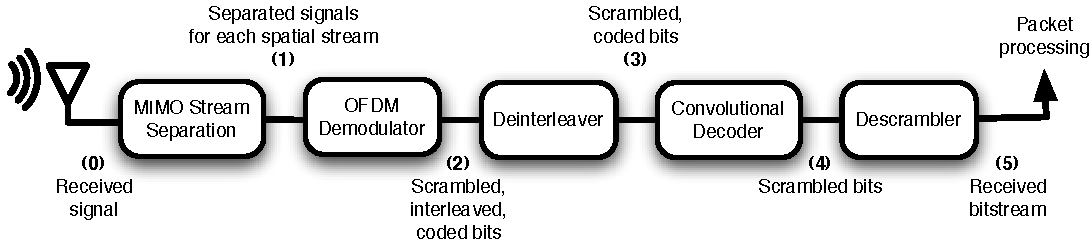
\includegraphics[width=6in]{figures/mimo_ofdm_decoding_process.pdf}
\caption{\label{fig:ofdm_decoding} The 802.11n MIMO-OFDM decoding process. MIMO receiver separates the RF signal~(0) for each spatial stream~(1). Demodulation converts the separated signals into bits~(2). Bits from the multiple streams are deinterleaved and combined~(3) followed by convolutional decoding~(4) to correct errors. Finally, scrambling that randomizes bit patterns is removed and the packet is processed~(5).}
\end{figure*}

\heading{Modeling Delivery.}
We build our model up from narrowband demodulation. 
Standard formulas summarized in \tabref{tab:ber_snr} relate SNR (denoted $\rho$) to bit-error rate (BER) for the modulations used in 802.11~\cite{Goldsmith}. CSI gives us the SNR values ($\rho_s$) to use for each subcarrier. For a SISO system, $\rho_s$ is given by the single entry in $H_s$.

In OFDM, decoding is applied across the demodulated bits of subcarriers. If we assume frequency-flat fading for the moment, then all the subcarriers have the same SNR\@. The link will behave the same as in our wired experiments in which RSSI reflect real performance and it will be easy to make predictions for a given SNR and modulation combination. We can use \figref{fig:snr_prr_attenuator} to measure the fixed transition points between rates and thus make our choice.

Frequency-selective fading complicates this picture as some weak subcarriers will be much more likely to have errors than others that are stronger. To model a link in this case, we turn to the notion of an \textbf{\em Effective SNR}. This is defined as the SNR that would give the \emph{same error performance on a narrowband channel}~\cite{nanda_effectiveSNR}. For example, the links in \figref{fig:example_fsf_shape} will have Effective SNR values that are nearly equal because they perform similarly, even though their RSSIs are spread over 15\dB.

The Effective SNR is \emph{not} simply the average subcarrier SNR; indeed, assuming a uniform noise floor, that average is indeed equivalent to the packet SNR derived from the RSSI\@. Instead, the Effective SNR is biased towards the weaker subcarrier SNRs because it is these subcarriers that produce most of the errors. If we ignore coding for the moment, then we can compute the Effective SNR by averaging the subcarrier BERs and then finding the corresponding SNR\@. That is:
\begin{equation}
\label{eq:effective_ber}
	\text{BER}_{\text{eff},k} = \frac{1}{52} \sum \text{BER}_k(\rho_s)
\end{equation}
\begin{equation}
\label{eq:effective_snr}
	\rho_{\text{eff},k} = \text{BER}_k^{-1}(\text{BER}_{\text{eff},k})
\end{equation}
We use $\text{BER}_k^{-1}$ to denote the inverse mapping, from BER to SNR\@. We have also called the average BER across subcarriers the effective BER, $\text{BER}_{\text{eff}}$. SoftRate estimates BER using internal receiver state~\cite{Vutukuru_SoftRate}. We compute it from channel measurements instead.

Note that the BER mapping and hence Effective SNR are functions of the modulation ($k$). That is, unlike the RSSI, a particular wireless channel will have four different Effective SNR values, one describing performance for each of the modulations. In practice, the interesting regions for the four Effective SNRs do not overlap because at a particular Effective SNR value only one modulation will be near the transition from useless (BER $\approx$0.5) to lossless (BER $\approx$0). When graphs in this paper are presented with an Effective SNR axis, we use all four values, each in the appropriate SNR range.

For 802.11n, we also model MIMO processing at the receiver. To do this we need to estimate the subcarrier SNRs for each spatial stream from the channel state matrix $H_s$. Although the standard does not specify receiver processing, 
we assume that a Minimum Mean Square Error (MMSE) receiver is used. It is computationally simple, optimal and equivalent to Maximal-Ratio Combining (MRC) for a single stream, and near optimal for multiple streams. 
All of these make it a likely choice in practice.
%This assumption allows us to use standard formulas to map channel matrices for each subcarrier (from CSI) to per-stream subcarrier SNRs.
%The $N$ per-stream MMSE output SNRs for subcarrier $s$ are 
The SNR of the $i^{\text{th}}$ stream after MMSE processing for subcarrier $s$ is 
given by $\rho_{s,i} = 1/Y_{ii}-1$, where
%\begin{equation}
%\label{eq:mmse_snr}
	$Y = \left(H_s^H H_s+I\right)^{-1}$
%\end{equation}
for $i \in [1,N]$ and $N$x$N$ identity matrix $I$~\cite{Tse}. For MIMO, the model computes the effective BER averaged across both subcarriers and streams.

Coding interacts with the notion of Effective SNR in a way that is difficult to analyze. One challenge is that the ability to correct bit errors depends on the position of the errors in the data stream. To sidestep this problem, we rely on the interleaving that randomizes the coded bits across subcarriers and spatial streams. Assuming perfect interleaving and robust coding, bit errors in the stream should look no different from bit errors for flat channels (but at a lower SNR). Thus our estimate of the effective BER in \eqref{eq:effective_ber} will accurately reflect the uncoded error performance of the link. Our algorithm now proceeds as in the case of a flat-fading channel described above: we take the computed Effective SNR value and use the measurements from a flat-fading link (\figref{fig:snr_prr_attenuator}) to determine transmission success or failure. As in CHARM~\cite{judd_rate_adapt}, we support different packet lengths with different SNR thresholds.

Note that this procedure differs from the typical approach of simulation-based analyses~\cite{Kant_fla, Liu_EESM, Nortel_3g}, that instead map the \emph{uncoded} BER estimate such as we compute to a \emph{coded} BER estimate by means of a simple log-linear approximation. They then use the coded BER estimate, and the length of the target transmission, to directly compute the packet delivery rate of the link. We believe our method of thresholding the Effective SNR is better because it directly accommodates variation in the receiver implementation. Different devices may have different \emph{noise figures}, a measure of how much signal strength is lost in the internal RF circuitry of the NIC\@. They may implement soft Viterbi decoders with more or fewer soft bits for their internal state, or indeed might do hard decoding instead. A receiver could use the optimal Maximum Likelihood MIMO decoder that has exponential complexity for small constellations like BPSK, but revert to the imperfect but more efficient MMSE at higher modulations. All of these can be easily expressed, albeit maybe approximately, as (perhaps modulation-dependent) shifts in the Effective SNR thresholds. In contrast, changing these parameters in the simulation approach involves changing the internals of the calculation.

\heading{Protocol Details.} Effective SNR calculations can be performed by either receiver or transmitter, and each has advantages. For it to make decisions, the transmitter must know the receiver's thresholds for the different rates; these are fixed for a particular model of NIC and can be shared once, e.g., during association. The transmitter also needs up-to-date CSI: either from feedback or estimated from the reverse path. Alternately, the receiver can request rates and select antennas directly using the new Link Adaptation Control field of any 802.11n QoS packet~\cite[\S7.1.3.5a]{80211n}. This obviates sending CSI, but the calculation instead requires that the transmitter share its spatial mappings, i.e. how it maps spatial streams to transmit antennas. These are likely to change less frequently than the channel, if at all. Finally, when operating in either mode with fewer transmit streams than antennas, the transmitter must occasionally send a short probe packet with all antennas to measure the full CSI\@.

\heading{Summary and Example.} Combining the above steps, our model consists of the following: 1) CSI is obtained and a test configuration is chosen; 2) the MMSE expression is used to compute per-stream, subcarrier SNRs from the CSI for the test number of streams; 3) the Effective SNR is computed from the per-stream, subcarrier SNRs for the test modulation; and 4) the Effective SNR is compared against the pre-determined threshold for the test modulation and coding to predict whether the link will deliver packets.

\begin{figure}[t]
  \centering
  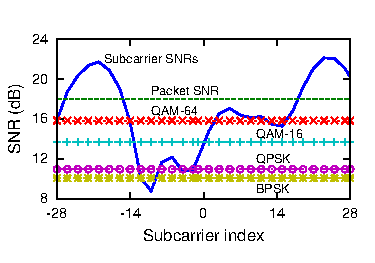
\includegraphics[width=0.9\columnwidth,viewport=0 9 180 111,clip]{figures/embed_fsf-shape-eff-snr-s3d5-txpower-20.pdf}
  % viewport=0 7 173 113
  \vspace{-4pt}
  \caption{Sample faded link showing the packet SNR and Effective SNRs for different modulations. BPSK has the lowest Effective SNR, but it needs less energy to decode.}
  \label{fig:eff_example}
  \vspace{-3pt}
\end{figure}


As an example, \figref{fig:eff_example} shows the CSI for a SISO link (steps 1--2) as a fading profile across subcarriers, with the computed Effective SNRs for all modulations (step 3). These Effective SNRs are compared with pre-determined thresholds (\figref{fig:snr_prr_attenuator}) to correctly predict that the best working rate will be 39\Mbps. 
Note that these Effective SNRs are well below the RSSI-based packet SNR that is biased towards the stronger subcarriers (note the logarithmic $y$-axis scale). This link does a poor job of harnessing the received power because it is badly faded, so its SNR is a poor predictor of rate.

\chapter{Application/Evaluation of Effective SNR}
\label{chap:esnr_eval}

\if 0
\begin{itemize}
\item Troubadour~\cite{halperin_troubadour}.
\item Power management~\cite{halperin_power}.
\item Channel measurement stuff that's cool.
\end{itemize}
\fi